\chapter*{Badania}

Celem tego rozdziału jest omówienie przeprowadzenej analizy oraz przedstawienie wyników klasyfikacji obrazów zwierząt dla modeli ResNet i ConvNeXt. Analiza ta obejmuje porównanie skuteczności modeli w różnych scenariuszach modyfikacji tła 
oraz w zależności od wielkości obiektu na obrazie oraz w zależności od predykowanej klasy.

\section*{Wyniki ogólne}

Badania miały na celu zbadanie wpływu modyfikacji tła na skuteczność klasyfikacji obrazów za pomocą dwóch wybranych modeli. W tym celu dokonano obliczeń podstawowych metryk, takich jak Accuracy, Precision, Recall i F1-score, dla oryginalnych 
oraz zmodyfikowanych obrazów, traktując wszystkie modyfikację jako jedną grupę.

Dla modelu ResNet, na oryginalnych obrazach uzyskano Accuracy na poziomie 0.886500, Precision 0.967026, Recall 0.886500 i F1-score 0.922742. Po modyfikacji tła wartości te uległy istotnemu obniżeniu, osiągając odpowiednio 0.697018 dla 
Accuracy, 0.948539 dla Precision, 0.697018 dla Recall i 0.802350 dla F1-score. W przypadku modelu ConvNeXt, na oryginalnych obrazach uzyskano wartości: Accuracy 0.943300, Precision 0.972519, Recall 0.943300 i F1-score 0.956791. Podobnie jak 
w przypadku ResNet, modyfikacja tła spowodowała obniżenie tych wartości, osiągając Accuracy 0.790873, Precision 0.961080, Recall 0.790873 i F1-score 0.866282. Ogólne wyniki można zaobserwować na \ref*{model_comparison_metrics} oraz \ref*{overall_metrics}

Analiza wyników wskazuje, że modyfikacja tła negatywnie wpływa na skuteczność obu modeli, jednak model o nowszej architekturze ConvNeXt wykazuje większą odporność na zmiany tła w porównaniu do modelu ResNet. Model ConvNeXt osiąga wyższe 
wartości metryk zarówno dla oryginalnych, jak i zmodyfikowanych obrazów, co sugeruje jego większą stabilność i lepszą adaptację do różnych warunków. Wartości metryk dla zmodyfikowanych obrazów są niższe w przypadku ResNet, co może 
wskazywać na większą wrażliwość tego modelu na zmiany w tle. Różnica w dokładności dla danych zmodyfikowanychwynosi aż 10 punktów procentowych, przy dokładności około 79 procent dla convnext oraz około 69 procent dla resnet. Model 
z nowszą architekturrą poradził sobie lepiej.

\begin{table}
	\centering
	\begin{tabular}{|c|c|c|c|c|c|}
		\hline
		\textbf{Model} & \textbf{Type} & \textbf{Accuracy} & \textbf{Precision} & \textbf{Recall} & \textbf{F1-score} \\
		\hline
		ResNet & Original & 0.886500 & 0.967026 & 0.886500 & 0.922742 \\
		\hline
		ResNet & Modified & 0.697018 & 0.948539 & 0.697018 & 0.802350 \\
		\hline
		ConvNeXt & Original & 0.943300 & 0.972519 & 0.943300 & 0.956791 \\
		\hline
		ConvNeXt & Modified & 0.790873 & 0.961080 & 0.790873 & 0.866282 \\
		\hline
	\end{tabular}
	\caption{Metryki porównawcze modeli ResNet i ConvNeXt}
	\label{tab:model_comparison_metrics}
\end{table}

Wyniki badań również wskazują, że pomimo modyfikacji tła, Precision dla obu modeli (ResNet i ConvNeXt) uległa jedynie niewielkiemu spadkowi. Mały spadek Precision w obu przypadkach sugeruje, że oba modele nadal skutecznie identyfikują 
prawdziwie pozytywne przypadki po modyfikacji tła.

\begin{figure}
	\centering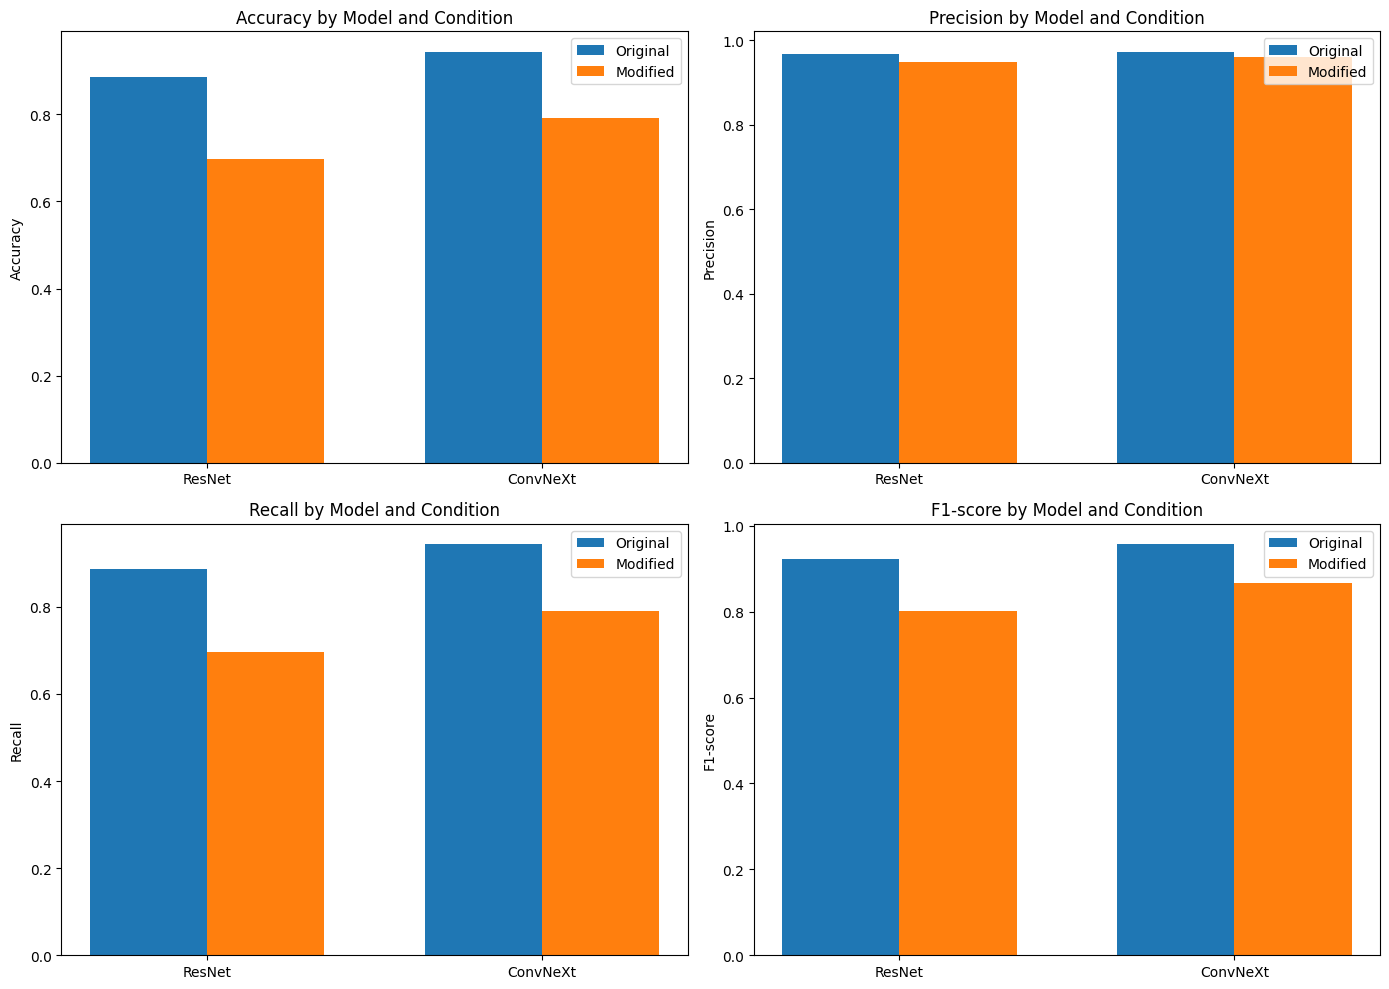
\includegraphics[width=.9\textwidth]{img/overall_metrics}
	\caption{Metryki dla danych oryginalnych zestawionych z danymi o zmodyfikowanych tłach}  
    \label{rys:overall_metrics}
\end{figure}


W badaniach obliczono również średnie wartości confidence scores w celu sprawdzenia pewności decyzji modeli. Wartości te obejmują ogólną średnią confidence score, a także średnie confidence scores dla poprawnych i niepoprawnych klasyfikacji. 
Dla modelu ResNet na oryginalnych obrazach średnia confidence score wyniosła 85.188854, ze średnią wartością 89.137424 dla poprawnych klasyfikacji i 54.348263 dla niepoprawnych. Po 
modyfikacji tła, średnia confidence score spadła do 71.694490, ze średnią wartością 83.929904 dla poprawnych klasyfikacji i 43.546579 dla niepoprawnych. Wyniki znajdują się w tabeli \ref*{model_confidence} oraz wizualizacja tych wyników na 
\ref*{confidence_avg}

W przypadku modelu ConvNeXt na oryginalnych obrazach średnia confidence score wyniosła 68.527975, ze średnią wartością 70.036361 dla poprawnych klasyfikacji i 43.433439 dla niepoprawnych. Po modyfikacji tła, średnia confidence score spadła 
do 57.543545, ze średnią wartością 63.189640 dla poprawnych klasyfikacji i 36.191272 dla niepoprawnych.

Wyniki te wskazują na znaczący spadek średnich confidence scores dla obu modeli po modyfikacji tła. Średnie confidence scores dla poprawnych klasyfikacji są wyższe niż dla niepoprawnych w obu przypadkach, co sugeruje, że modele są bardziej 
pewne swoich poprawnych klasyfikacji. Jednak modyfikacja tła powoduje ogólny średni spadek pewności modeli. 

Analiza wartości confidence scores dla ConvNeXt wskazuje na większy spadek w porównaniu do modelu ResNet. Ciekawe jest, że mimo większej dokładności predykcji, model convnext posiada znacznie niższe wartości confidence score. 

Podsumowując, modyfikacja tła ma w tym przypadku wyraźny wpływ na zmniejszenie pewności klasyfikacji obrazów przez oba modele. Chociaż oba modele wykazują wysoką pewność przy poprawnych klasyfikacjach, modyfikacja tła powoduje ogólny spadek 
tych wartości, z bardziej zauważalnym spadkiem w przypadku modelu ConvNeXt. 

\begin{table}
	\centering
	\begin{tabular}{|c|c|c|c|c|c|}
		\hline
		\textbf{Model} & \textbf{Type} & \textbf{Average} & 
		\textbf{Average correct} & \textbf{Average incorrect} \\
		\hline
		ResNet & Original & 85.188854 & 89.137424 & 54.348263 \\
		\hline
		ResNet & Modified & 71.694490 & 83.929904 & 43.546579  \\
		\hline
		ConvNeXt & Original & 68.527975 & 70.036361 & 43.433439 \\
		\hline
		ConvNeXt & Modified & 57.543545 & 63.189640 & 36.191272 \\
		\hline
	\end{tabular}
	\caption{Confidence scores dla modeli ResNet i ConvNeXt}
	\label{tab:model_confidence}
\end{table}

\begin{figure}
	\centering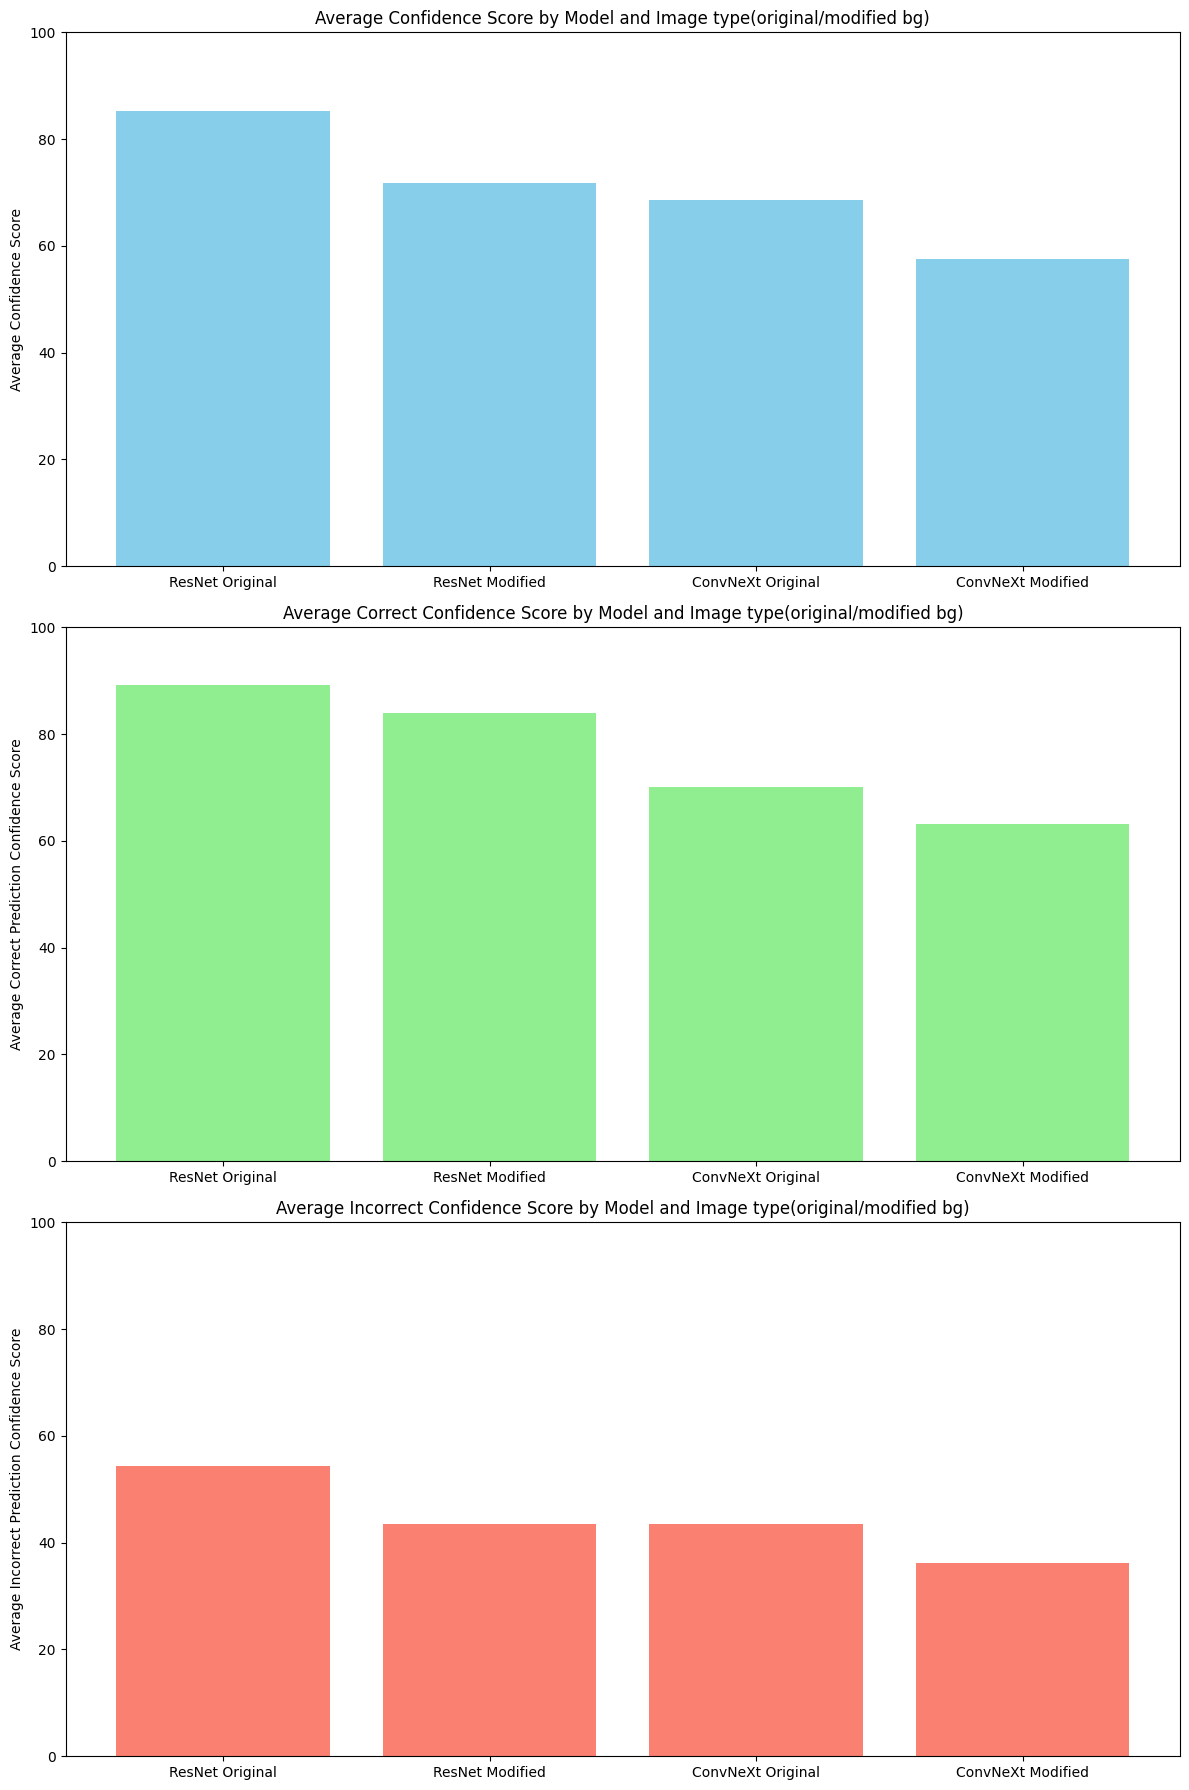
\includegraphics[width=.9\textwidth]{img/confidence_avg}
	\caption{Średnie wartości dla confidence scores}  
    \label{rys:confidence_avg}
\end{figure}
\newpage
Na podstawie dystrybucji confidence scores widocznynch na rysunkach \ref*{res_c_distro} oraz \ref*{conv_c_distro} dla modeli ResNet i ConvNeXt można wyciągnąć kilka istotnych wniosków. Model ResNet wykazuje wysoką pewność dla poprawnych 
klasyfikacji, co wskazuje na jego stabilność w identyfikowaniu prawidłowych przypadków. W przypadku błędnych klasyfikacji confidence scores są bardziej równomiernie rozłożone, co oznacza, że model jest mniej pewny, gdy się myli. Z kolei 
model ConvNeXt ma szerszy rozkład confidence scores, większość poprawnych klasyfikacji znajduje się w przedziale 70-80 i dla błędnych w przedziale 30-40. Mimo mniejszej pewności model convnext odnotował mniejsze spadki pewności w porównaniu
z pewnością na zdjęciach oryginalnych. Można z tego wnioskować, że modyfikacje tła mniej wpływają na pewność modelu convnext niż na resnet.

\begin{figure}
	\centering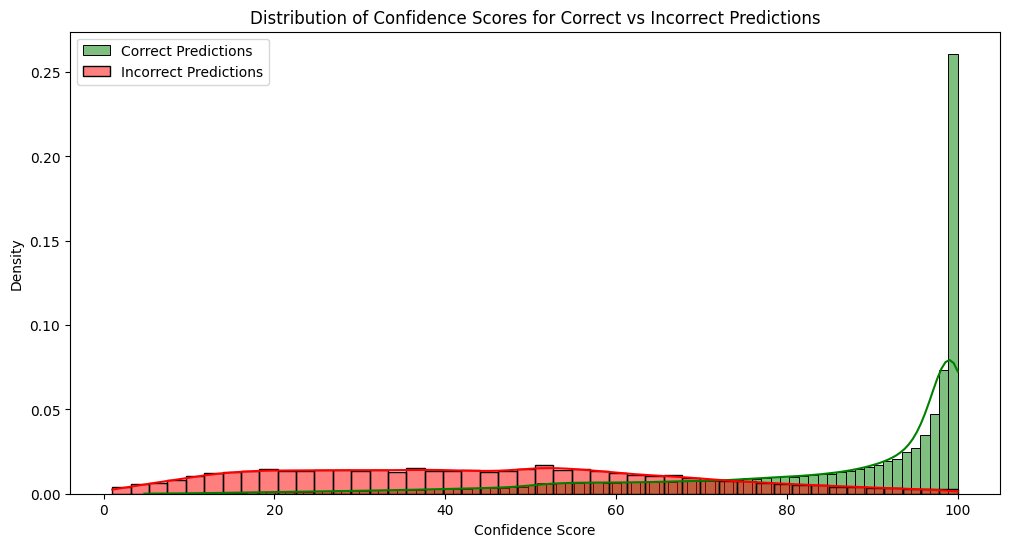
\includegraphics[width=.9\textwidth]{img/resnet_conf_distro}
	\caption{Dystrybucja confidence score dla ResNet}
	\label{rys:res_c_distro}
\end{figure}

\begin{figure}
	\centering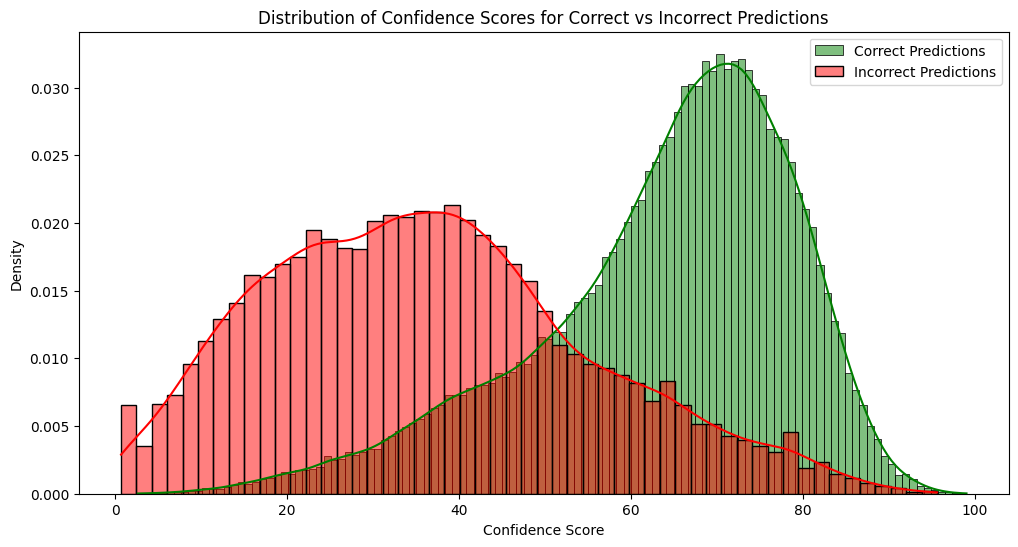
\includegraphics[width=.9\textwidth]{img/convnext_conf_distro}
	\caption{Dystrybucja confidence score dla ConvNext}
	\label{rys:conv_c_distro}
\end{figure}
\newpage

\section*{Wyniki względem kategorii wielkości obiektu}

Kolejną częścia analizy było zbadanie metryk modeli w kontekście różnych rozmiarów obiektu na zdjęciu. Analiza wpływu wielkości obiektu na skuteczność klasyfikacji obrazów jest istotnym elementem badań, ponieważ różne rozmiary obiektów mogą 
znacząco wpływać na wydajność modeli głębokiego uczenia. Zdjęcia z obiektami o różnych wielkościach mogą być różnie traktowane przez modele klasyfikacyjne ze względu na różną ilość "zakłóceń" jakim jest tło. Dlatego też, zrozumienie, jak 
zmienia się dokładność modeli ResNet i ConvNeXt w zależności od wielkości obiektu, jest kluczowe dla optymalizacji i poprawy tych modeli w rzeczywistych zastosowaniach.



\begin{table}
	\centering
	\begin{tabular}{|c|c|c|c|c|c|}
		\hline
		\textbf{Object Size} & \textbf{Dataset Type} & \textbf{Accuracy} & \textbf{Precision} & \textbf{Recall} & \textbf{F1-score} \\
		\hline
		Large & Original & 0.877353 & 0.972679 & 0.877353 & 0.920111 \\
		\hline
		Large & Modified & 0.789338 & 0.960967 & 0.789338 & 0.865607 \\
		\hline
		Medium & Original & 0.897879 & 0.963620 & 0.897879 & 0.927600 \\
		\hline
		Medium & Modified & 0.762727 & 0.943926 & 0.762727 & 0.841553 \\
		\hline
		Small & Original & 0.884545 & 0.963823 & 0.884545 & 0.918217 \\
		\hline
		Small & Modified & 0.552828 & 0.935458 & 0.552828 & 0.686206 \\
		\hline
	\end{tabular}
	\caption{Metryki porównawcze modelu ResNet w zależności od wielkości obiektu}
	\label{tab:resnet_object_size_metrics}
\end{table}

Dla modelu ResNet wyniki pokazują, że dla dużych obiektów na oryginalnych obrazach uzyskano Accuracy na poziomie 0.877353, Precision 0.972679, Recall 0.877353 i F1-score 0.920111. Po modyfikacji tła wartości te spadły odpowiednio do 
0.789338, 0.960967, 0.789338 i 0.865607. Dla obiektów średniej wielkości na oryginalnych obrazach uzyskano Accuracy 0.897879, Precision 0.963620, Recall 0.897879 i F1-score 0.927600, a po modyfikacji tła wartości te spadły do 0.762727, 
0.943926, 0.762727 i 0.841553. Dla małych obiektów na oryginalnych obrazach uzyskano Accuracy 0.884545, Precision 0.963823, Recall 0.884545 i F1-score 0.918217, natomiast po modyfikacji tła wartości te drastycznie spadły do 0.552828, 0.935458, 
0.552828 i 0.686206.

Dla modelu ConvNeXt wyniki pokazują, że dla dużych obiektów na oryginalnych obrazach uzyskano Accuracy na poziomie 0.932353, Precision 0.974247, Recall 0.932353 i F1-score 0.952076. Po modyfikacji tła wartości te spadły odpowiednio do 
0.846397, 0.970483, 0.846397 i 0.902546. Dla obiektów średniej wielkości na oryginalnych obrazach uzyskano Accuracy 0.943333, Precision 0.970287, Recall 0.943333 i F1-score 0.955907, a po modyfikacji tła wartości te spadły do 0.840682, 
0.959570, 0.840682 i 0.892625. Dla małych obiektów na oryginalnych obrazach uzyskano Accuracy 0.954545, Precision 0.972766, Recall 0.954545 i F1-score 0.961567, natomiast po modyfikacji tła wartości te spadły do 0.705480, 0.950400, 0.705480 i 
0.804351.

\begin{table}
	\centering
	\begin{tabular}{|c|c|c|c|c|c|}
		\hline
		\textbf{Object Size} & \textbf{Dataset Type} & \textbf{Accuracy} & \textbf{Precision} & \textbf{Recall} & \textbf{F1-score} \\
		\hline
		Large & Original & 0.932353 & 0.974247 & 0.932353 & 0.952076 \\
		\hline
		Large & Modified & 0.846397 & 0.970483 & 0.846397 & 0.902546 \\
		\hline
		Medium & Original & 0.943333 & 0.970287 & 0.943333 & 0.955907 \\
		\hline
		Medium & Modified & 0.840682 & 0.959570 & 0.840682 & 0.892625 \\
		\hline
		Small & Original & 0.954545 & 0.972766 & 0.954545 & 0.961567 \\
		\hline
		Small & Modified & 0.705480 & 0.950400 & 0.705480 & 0.804351 \\
		\hline
	\end{tabular}
	\caption{Metryki porównawcze modelu ConvNeXt w zależności od wielkości obiektu}
	\label{tab:convnext_object_size_metrics}
\end{table}

Analiza wyników pokazuję, że wielkośc obiektu ma znaczący wpływ na jakość klasyfikacji, mianowicie im mniejszy obiekt tym większe większe pogorszenie metryk modeli. Oba modele uzyskały największe pogorszenie metryk dla najmniejszych obiektów oraz 
okazały się najbardziej odporne przy największych obiektach, co jest dosyć logicznym procesem, ponieważ przy dużych obiektach jest mniej zakłóceń na zdjęciu w postaci tła. Model convnext okazał się bardziej odporny, w każdej kategorii wielkości
odnotował mniejsze spadki niż resnet.


Wyniki te podkreślają znaczenie rozważania wielkości obiektów przy problemach klasyfikacyjnych. Modele mogą wymagać dodatkowego dostrajania lub augmentacji danych, aby poprawić ich odporność na zmiany tła, co jest 
szczególnie istotne dla zastosowań, gdzie obiekty mogą występować w różnych skalach i warunkach środowiskowych. Zrozumienie, że większy udział tła przy małych obiektach może prowadzić do większych zakłóceń, jest kluczowe dla opracowywania 
bardziej efektywnych algorytmów klasyfikacyjnych, które mogą niezawodnie działać w zmiennych warunkach.

\begin{table}
	\centering
	\begin{tabular}{|c|c|c|c|}
		\hline
		\textbf{Object Size} & \textbf{Average Score} & \textbf{Correct Score} & \textbf{Incorrect Score} \\
		\hline
		Large & 76.790632 & 85.228727 & 43.843488 \\
		\hline
		Medium & 76.564846 & 85.185492 & 47.188400 \\
		\hline
		Small & 65.356645 & 82.693992 & 41.576619 \\
		\hline
	\end{tabular}
	\caption{Confidence scores dla modelu ResNet w zależności od wielkości obiektu oraz poprawności predykcji}
	\label{tab:resnet_confidence_scores}
\end{table}

\begin{table}
	\centering
	\begin{tabular}{|c|c|c|c|}
		\hline
		\textbf{Object Size} & \textbf{Average Score} & \textbf{Correct Score} & \textbf{Incorrect Score} \\
		\hline
		Large & 64.332577 & 69.300610 & 35.502391 \\
		\hline
		Medium & 60.275503 & 64.107149 & 38.802715 \\
		\hline
		Small & 50.455171 & 56.473165 & 34.618265 \\
		\hline
	\end{tabular}
	\caption{Confidence scores dla modelu ConvNeXt w zależności od wielkości obiektu oraz poprawności predykcji}
	\label{tab:convnext_confidence_scores}
\end{table}

Dla modelu ResNet, średnie confidence scores wynoszą 76.790632 dla dużych obiektów, 76.564846 dla obiektów średniej wielkości i 65.356645 dla małych obiektów. Dla poprawnych klasyfikacji confidence scores są odpowiednio wyższe, wynosząc 
85.228727, 85.185492 i 82.693992. Dla niepoprawnych klasyfikacji wartości te są znacznie niższe: 43.843488, 47.188400 i 42.576619.

W przypadku modelu ConvNeXt, średnie confidence scores są niższe i wynoszą 64.332577 dla dużych obiektów, 60.275503 dla obiektów średniej wielkości i 50.455171 dla małych obiektów. Confidence scores dla poprawnych klasyfikacji wynoszą 
69.300610, 64.107149 i 56.473165, a dla niepoprawnych klasyfikacji są to 35.502391, 38.802715 i 34.618265.

Wraz ze wzrostem wielkości obiektu na badanych zdjęcia wzrasta pewność obu modeli. Największy spadek pewności występuje dla małych obiektów.

Porównując oba modele, ResNet wykazuje wyższe średnie confidence scores zarówno dla poprawnych, jak i niepoprawnych klasyfikacji w porównaniu do ConvNeXt. To sugeruje, że ResNet jest bardziej pewny swoich decyzji, niezależnie od wielkości 
obiektu.

\section*{Wyniki względem typu modyfikacji tła}

W tej sekcji przeanalizowano wpływ różnych typów modyfikacji tła na skuteczność klasyfikacji obrazów. Obliczono również podstawowe metryki, pewności predykcji oraz przedstawiono macierze korelacji dla obu modeli. 

\begin{table}
    \centering
    \begin{tabular}{|c|c|c|c|c|}
        \hline
        \textbf{Modification Type} & \textbf{Accuracy} & \textbf{Precision} & \textbf{Recall} & \textbf{F1-score} \\
        \hline
        Desert & 0.7582 & 0.956658 & 0.7582 & 0.844717 \\
        \hline
        Low Contrast & 0.7835 & 0.957333 & 0.7835 & 0.859445 \\
        \hline
        City & 0.7620 & 0.955729 & 0.7620 & 0.845955 \\
        \hline
        Sky & 0.7577 & 0.951998 & 0.7577 & 0.840614 \\
        \hline
        Jungle & 0.7736 & 0.952716 & 0.7736 & 0.846911 \\
        \hline
        No Background & 0.7629 & 0.948944 & 0.7629 & 0.843935 \\
        \hline
        High Contrast & 0.7757 & 0.952540 & 0.7757 & 0.852606 \\
        \hline
        No Foreground & 0.1935 & 0.857598 & 0.1935 & 0.260654 \\
        \hline
        Water & 0.7198 & 0.950886 & 0.7198 & 0.812003 \\
        \hline
        Snow & 0.7462 & 0.961568 & 0.7462 & 0.833842 \\
        \hline
        Indoor & 0.6990 & 0.950477 & 0.6990 & 0.801644 \\
        \hline
        Mountain & 0.6980 & 0.959372 & 0.6980 & 0.800749 \\
        \hline
    \end{tabular}
    \caption{Metryki według typu modyfikacji dla ResNet}
    \label{tab:resnet_metrics_modification}
\end{table}

\begin{table}
	\centering
	\begin{tabular}{|c|c|c|c|}
		\hline
		\textbf{Modification Type} & \textbf{Average Score} & \textbf{Correct Score} & \textbf{Incorrect Score} \\
		\hline
		Desert & 75.954396 & 84.304869 & 49.770241 \\
		\hline
		Low Contrast & 77.879677 & 86.411184 & 47.004688 \\
		\hline
		City & 73.458863 & 84.253234 & 38.898736 \\
		\hline
		Sky & 76.063737 & 84.893389 & 48.452397 \\
		\hline
		Jungle & 77.082096 & 85.830222 & 47.190088 \\
		\hline
		No Background & 74.429546 & 85.308617 & 39.424725 \\
		\hline
		High Contrast & 77.275950 & 86.369482 & 45.827655 \\
		\hline
		No Foreground & 41.084428 & 67.091235 & 34.844729 \\
		\hline
		Water & 70.044268 & 80.529769 & 43.108282 \\
		\hline
		Snow & 76.379893 & 85.181503 & 50.502187 \\
		\hline
		Indoor & 72.859840 & 83.005442 & 49.299121 \\
		\hline
		Mountain & 70.556246 & 82.283334 & 43.451917 \\
		\hline
	\end{tabular}
	\caption{Confidence scores dla modelu ResNet według typu modyfikacji}
	\label{tab:resnet_confidence_scores_modification}
\end{table}

\begin{table}
	\centering
	\begin{tabular}{|c|c|c|c|c|}
		\hline
		\textbf{Modification Type} & \textbf{Accuracy} & \textbf{Precision} & \textbf{Recall} & \textbf{F1-score} \\
		\hline
		Desert & 0.8234 & 0.965246 & 0.8234 & 0.885689 \\
		\hline
		Low Contrast & 0.8897 & 0.965665 & 0.8897 & 0.925404 \\
		\hline
		City & 0.8392 & 0.967133 & 0.8392 & 0.894941 \\
		\hline
		Sky & 0.8259 & 0.958754 & 0.8259 & 0.886533 \\
		\hline
		Jungle & 0.8621 & 0.963912 & 0.8621 & 0.909624 \\
		\hline
		No Background & 0.8765 & 0.961364 & 0.8765 & 0.915996 \\
		\hline
		High Contrast & 0.8707 & 0.964345 & 0.8707 & 0.913518 \\
		\hline
		No Foreground & 0.2572 & 0.921080 & 0.2572 & 0.343413 \\
		\hline
		Water & 0.8593 & 0.960770 & 0.8593 & 0.906849 \\
		\hline
		Snow & 0.8567 & 0.966667 & 0.8567 & 0.902537 \\
		\hline
		Indoor & 0.7797 & 0.965780 & 0.7797 & 0.859119 \\
		\hline
		Mountain & 0.8357 & 0.964700 & 0.8357 & 0.891118 \\
		\hline
	\end{tabular}
	\caption{Metryki według typu modyfikacji dla ConvNeXt}
	\label{tab:convnext_metrics_modification}
\end{table}

\begin{table}
	\centering
	\begin{tabular}{|c|c|c|c|}
		\hline
		\textbf{Modification Type} & \textbf{Average Score} & \textbf{Correct Score} & \textbf{Incorrect Score} \\
		\hline
		Desert & 61.750625 & 65.260020 & 45.388021 \\
		\hline
		Low Contrast & 57.798021 & 61.428446 & 28.514347 \\
		\hline
		City & 58.404538 & 62.933008 & 34.770883 \\
		\hline
		Sky & 56.927464 & 60.928925 & 37.945228 \\
		\hline
		Jungle & 60.313014 & 63.350853 & 41.321559 \\
		\hline
		No Background & 57.877617 & 62.096968 & 27.932186 \\
		\hline
		High Contrast & 57.146265 & 61.220278 & 29.712060 \\
		\hline
		No Foreground & 38.674228 & 56.533386 & 32.490362 \\
		\hline
		Water & 57.189347 & 60.885762 & 34.614159 \\
		\hline
		Snow & 61.818994 & 65.527449 & 39.648495 \\
		\hline
		Indoor & 61.650110 & 66.519692 & 44.415372 \\
		\hline
		Mountain & 61.306386 & 66.316218 & 35.824236 \\
		\hline
	\end{tabular}
	\caption{Confidence scores dla modelu ConvNeXt według typu modyfikacji}
	\label{tab:convnext_confidence_scores_modification}
\end{table}

Analiza wyników pokazuje, że typ modyfikacji tła ma znaczący wpływ na skuteczność klasyfikacji obrazów oraz wartości confidence scores dla obu modeli. Oba modele osiągały najlepsze wyniki głównie na modyfikacjach, które były jednokolorowe, a mianowicie na "no\_background", "high\_contrast"
oraz "low\_contrast". W pierwszym przypadku tło było całkowicie czarne, a w pozostałych kolor był dobrany na podstawie dominujących kolorów w obiektach danej klasy. Najlepsze wyniki oba modele uzyskały na tle o kolorze niskokontrastowym do obiektu. Zarówno ResNet jak i ConvNext
osiągneły nieco gorsze wyniki dla sceneri wodnej, wnętrza domu oraz scenerii górzystej. Dokładne wartośći można zaobserwawać w tabelach \ref*{resnet_confidence_scores_modification} oraz \ref*{convnext_metrics_modification}. Wyższa dokładność na modyfikacjach jednokolorowych prawdopodobnie wynika z powodu mniejszej liczby elementów na 
zdjęciach, które mogą być mylące dla modeli. Oba modele poardziły sobie fatalnie w sytuacji gdy ze zdjęcia został usunięty obiekt i pozostawione zostało tło, jednak model ConvNext był bardziej odporny i lepiej radził sobie z analizowaniem samego pozostawionego kształtu obiektu. Dla modelu
ConvNeXt jedyną modyfikacją (poza usunięciem obiektu), na której uzyskał wartość dokładnośći poniżej 80 \% jest sceneria z wnętrznem domu. Wysoką wartość accuracy uzyskała również sceneria dżungli dla obu modeli, może to wynikać z faktu iż ta sceneria posiada dużo zielonych roślin,
które często mogą występować przy rzeczywistych zdjęciach wybranych zwierząt.

Jeżeli chodzi o pewnośc modeli co do swoich decyzji to, dla modelu ResNet oscylowała w okolicach 70-75 \% dla wszystkich modyfikacji, poza scenariuszem usunięcia obiektu ze zdjęcia gdzie wyniosła 40 \%. Model ConvNext posiada mniejszą pewność, która wynosi około 60 \% oraz 40 \% dla 
sytuacji bez obiektu.

Wyniki te podkreślają znaczenie uwzględniania różnych typów tła podczas trenowania i oceny modeli klasyfikacyjnych. Zrozumienie, jak różne modyfikacje tła wpływają na skuteczność i pewność klasyfikacji, może prowadzić do opracowania bardziej odpornych modeli, które lepiej radzą 
sobie w zróżnicowanych warunkach. Dalsze badania mogą skoncentrować się na metodach augmentacji danych, które mogą poprawić wydajność modeli w scenariuszach z różnorodnymi tłami. Tła o mniejszej ilości rozpraszających elementów lub te przypominające naturalne warunki występowania zwięrzat
na rzeczywistych zdjęciach radziły sobie lepiej z problemem klasyfikacji. 

\section*{Wyniki względem klas}

W niniejszym podrozdziale przedstawiono wyniki badań dotyczących wpływu tła na skuteczność klasyfikacji względem już konkretnych klas. W tych badaniach skupiono się na analizie średniej dokładności oraz średniej pewności względem typu modyfiakcji dla każdej klasy osobno. Sprawdzano 
również jakie błędy są najczęściej podejmowane, czyli z jaką klasą jest najczęściej mylona. Badania obejmowały analizę dziesięciu różnych klas obiektów, takich jak "ram, tup", "Greater Swiss Mountain dog", "hummingbird", "Egyptian cat", "bighorn sheep", "Old English sheepdog", 
"Persian cat", "junco, snowbird", "German shepherd" i "American robin". Klasy te reprezentują trzy rasy psów, dwie rasy kotów, trzy rasy ptaków oraz dwie rasy owiec. 

\section*{Wnioski dla klasy 348 (ram, tup)}

Na podstawie wyników dwóch modeli przedstawionych w \ref*{metrics_confidence_class_348_resnet} i \ref*{metrics_confidence_class_348_convnext}, można wyciągnąć następujące wnioski dotyczące wpływu różnych 
modyfikacji tła na klasyfikację klasy 348 (ram, tup) przy użyciu modeli ResNet i ConvNeXt:

\subsection*{Model ResNet}

Model ResNet osiągnął dosyć niską dokładność 0.781 na oryginalnych obrazach, co wskazuje na dosyć problematyczną klasę. Średnia pewność wynosiła 80.888742, co jest stosunkowo wysoką wartością, potwierdzającą pewność modelu przy klasyfikacji. Najczęściej myloną klasą była klasa 
"Bighorn sheep" dla wszystkich typów modyfikacji. Te dwie klasy są niemal identyczne nawet dla ludzkiego oka, co można zaobserwować na \ref*{348}.

Dla większości modyfikacji wartości accuracy się obniżyły. Dla jednego typu modyfikacji udało się polepszeć metrykę dokładności o około 5 punktów procentowych, a mianowicie dla scenerii dżungli. Największe spadki uzsykano dla scenerii górzystych i śnieżnych, dla których znacznie wzrosła
liczba przypadków gdzie pomylono się z klasą "bighorn sheep". Podejrzewam, że tereny górzyste czy śnieżne są miejscem, w którym klasa "bighorn sheep" znajduję się częsciej niż przewidywana klasa "ram, tup", natomiast sceneria dżungli pomaga modelowi rozróżnić te dwie klasy, gdzie
liczba pomyłek jest znacznie niższa.


\begin{figure}
	\centering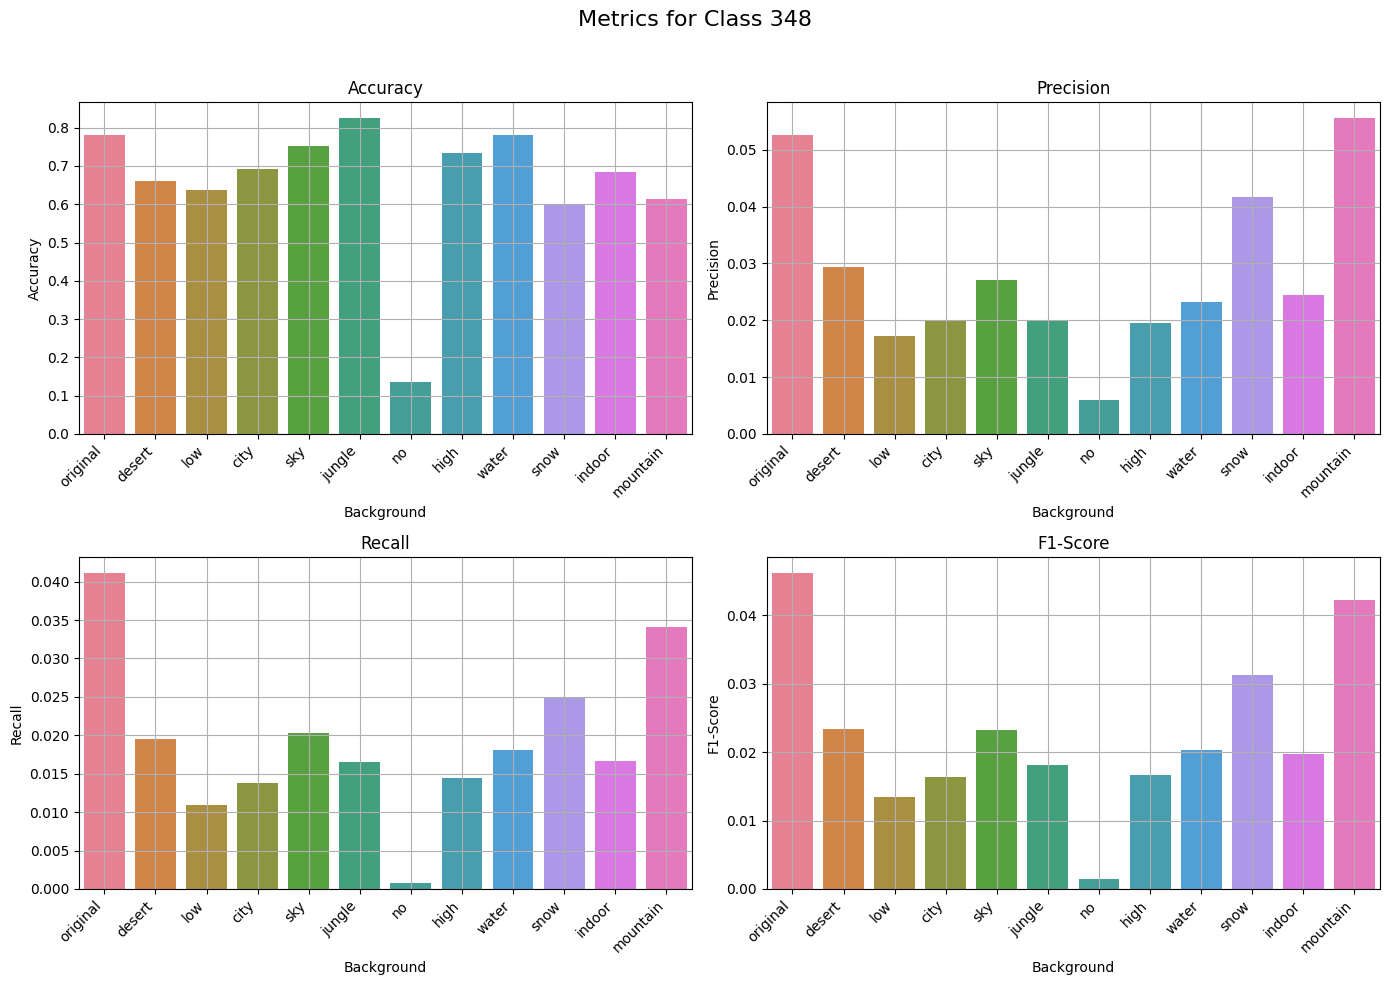
\includegraphics[width=.9\textwidth]{img/348}
	\caption{Po lewej "ram, tup" (true\_class), natomiast po prawej "bighorn sheep"}
	\label{rys:348}
\end{figure}

\subsection*{Model ConvNeXt}

Model ConvNeXt osiągnął nieco wyższą dokładność dla oryginalnych zdjęć niż ResNet, lecz nie udało się uzyskać lepszych metryk dla żadnej modyfikacji. Spośród modyfikacji wyniki również były najlepsze dla scenerii dżungli oraz wody, podobnie jak dla wcześniejszego modelu. Relatywnie 
wysokie wartości uzyskano także dla tła o niskim kontraście. Ten model zdecydowanie był bardziej wrażliwy na modyfikację tła, ponieważ w większej liczbie kategorii uzyskał znacznie gorsze wyniki. Więcej typów modyfikacji przyczyniło się do pomyłki z klasą "bighorn sheep". 

\begin{table}
	\centering
	\begin{tabular}{|c|c|c|c|}
		\hline
		\textbf{Modification Type} & \textbf{Accuracy} & \textbf{Avg Confidence} & \textbf{Most Mistaken} \\
		\hline
		Original & 0.781 & 80.888742 & Bighorn, bighorn sheep (194) \\
		\hline
		Desert & 0.662 & 73.618091 & Bighorn, bighorn sheep (212) \\
		\hline
		Low Contrast & 0.637 & 72.533478 & Bighorn, bighorn sheep (241) \\
		\hline
		City & 0.691 & 71.055787 & Bighorn, bighorn sheep (175) \\
		\hline
		Sky & 0.752 & 74.196770 & Bighorn, bighorn sheep (125) \\
		\hline
		Jungle & 0.825 & 76.201070 & Bighorn, bighorn sheep (84) \\
		\hline
		No Background & 0.668 & 71.519892 & Bighorn, bighorn sheep (213) \\
		\hline
		High Contrast & 0.735 & 73.587178 & Bighorn, bighorn sheep (163) \\
		\hline
		No Foreground & 0.136 & 38.340821 & American black bear, black bear (137) \\
		\hline
		Water & 0.780 & 72.729140 & Bighorn, bighorn sheep (97) \\
		\hline
		Snow & 0.601 & 76.547279 & Bighorn, bighorn sheep (318) \\
		\hline
		Indoor & 0.683 & 71.596914 & Bighorn, bighorn sheep (132) \\
		\hline
		Mountain & 0.613 & 74.327448 & Bighorn, bighorn sheep (285) \\
		\hline
	\end{tabular}
	\caption{Metrics and Confidence Scores for Class 348 (ram, tup) - ResNet}
	\label{tab:metrics_confidence_class_348_resnet}
\end{table}

\begin{table}
	\centering
	\begin{tabular}{|c|c|c|c|}
		\hline
		\textbf{Modification Type} & \textbf{Accuracy} & \textbf{Avg Confidence} & \textbf{Most Mistaken} \\
		\hline
		Original & 0.801 & 64.573134 & Bighorn, bighorn sheep (191) \\
		\hline
		Desert & 0.589 & 59.293923 & Bighorn, bighorn sheep (305) \\
		\hline
		Low Contrast & 0.752 & 57.574512 & Bighorn, bighorn sheep (211) \\
		\hline
		City & 0.604 & 57.563126 & Bighorn, bighorn sheep (311) \\
		\hline
		Sky & 0.717 & 57.364283 & Bighorn, bighorn sheep (204) \\
		\hline
		Jungle & 0.747 & 60.548807 & Bighorn, bighorn sheep (187) \\
		\hline
		No Background & 0.703 & 56.948889 & Bighorn, bighorn sheep (236) \\
		\hline
		High Contrast & 0.706 & 56.227286 & Bighorn, bighorn sheep (244) \\
		\hline
		No Foreground & 0.274 & 36.891416 & American black bear, black bear (151) \\
		\hline
		Water & 0.745 & 57.906020 & Bighorn, bighorn sheep (202) \\
		\hline
		Snow & 0.580 & 59.995922 & Bighorn, bighorn sheep (371) \\
		\hline
		Indoor & 0.556 & 59.476196 & Bighorn, bighorn sheep (288) \\
		\hline
		Mountain & 0.588 & 61.288639 & Bighorn, bighorn sheep (345) \\
		\hline
	\end{tabular}
	\caption{Metrics and Confidence Scores for Class 348 (ram, tup) - ConvNeXt}
	\label{tab:metrics_confidence_class_348_convnext}
\end{table}

\section*{Wnioski dla klasy 238 (Greater Swiss Mountain dog)}

Na podstawie wyników dwóch modeli przedstawionych w \ref*{metrics_confidence_class_238_resnet} i \ref*{metrics_confidence_class_238_convnext}, można wyciągnąć następujące wnioski dotyczące wpływu różnych 
modyfikacji tła na klasyfikację klasy 238 (Greater Swiss Mountain dog) przy użyciu modeli ResNet i ConvNeXt:

\subsection*{Model ResNet}

Dla modelu ResNet udało się minimalnie polepszyć wyniki klasyfikacji dla trzech scenerii: pustynnej, śnieżnej oraz wnętrza domu, dla reszty modyfikacji wyniki były gorsze. Model najczęściej mylił się z dwoma klasami, w zależności od typu modyfikacji. Wszystkie trzy klasy są bardzo do siebie
podobne co można zaobserwować na rysunku \ref*{238}  

\begin{figure}
	\centering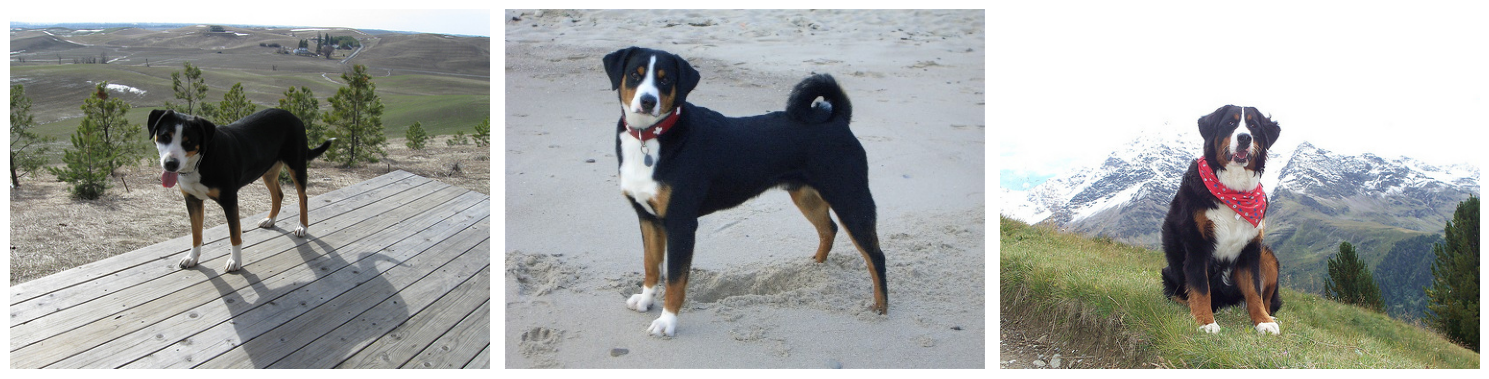
\includegraphics[width=.9\textwidth]{img/238}
	\caption{Od lewej "Greater Swiss Mountain dog" (true\_class), "Appenzeller", "EntleBucher"}
	\label{rys:238}
\end{figure}

\subsection*{Model ConvNeXt}

Model o nowszej architekturze znacznie lepiej poradził sobie w przypadku tej klasy. Wynik dokładności polepszył się o około 15 punktów procentowych. Jeżeli chodzi o modyfiakcje, to dla wszystkich uzyskano gorsze wyniki, szczególnie dla scenerii nieba oraz modyfikacji o wysokim kontraście, gdzie
metryki spadły poniżej 80\%. Podobnie jak wcześniej najczęstsze pomyłki dzieliły się między podobne rasy psów Appenzeller oraz EntleBucher. Ciekawym zjawiskiem jest najczęstsza pomyłka tego modelu dla scenerii wnętrza domu, gdzie model najczęściej mylił sie klasyfikując zdjęcie jako
półkę z książkami. Dowodzi to że różne niechciane obiekty znajdujące się w tle mogą zakłócać proces klasyfikacji. 

\begin{table}
	\centering
	\begin{tabular}{|c|c|c|c|}
		\hline
		\textbf{Modification Type} & \textbf{Accuracy} & \textbf{Avg Confidence} & \textbf{Most Mistaken} \\
		\hline
		Original & 0.746 & 69.254460 & EntleBucher (83) \\
		\hline
		Desert & 0.751 & 71.670600 & EntleBucher (71) \\
		\hline
		Low Contrast & 0.628 & 66.772043 & EntleBucher (168) \\
		\hline
		City & 0.720 & 70.455594 & Appenzeller (79) \\
		\hline
		Sky & 0.693 & 67.656871 & EntleBucher (103) \\
		\hline
		Jungle & 0.680 & 66.612556 & EntleBucher (99) \\
		\hline
		No Background & 0.675 & 66.545953 & EntleBucher (114) \\
		\hline
		High Contrast & 0.632 & 65.697515 & Appenzeller (118) \\
		\hline
		No Foreground & 0.009 & 29.458587 & American black bear, black bear (69) \\
		\hline
		Water & 0.679 & 65.613398 & Appenzeller (97) \\
		\hline
		Snow & 0.748 & 71.034704 & EntleBucher (96) \\
		\hline
		Indoor & 0.750 & 71.739733 & Appenzeller (57) \\
		\hline
		Mountain & 0.605 & 63.748537 & EntleBucher (165) \\
		\hline
	\end{tabular}
	\caption{Metrics and Confidence Scores for Class 238 (Greater Swiss Mountain dog) - ResNet}
	\label{tab:metrics_confidence_class_238_resnet}
\end{table}

\begin{table}
	\centering
	\begin{tabular}{|c|c|c|c|}
		\hline
		\textbf{Modification Type} & \textbf{Accuracy} & \textbf{Avg Confidence} & \textbf{Most Mistaken} \\
		\hline
		Original & 0.918 & 67.297499 & EntleBucher (30) \\
		\hline
		Desert & 0.812 & 53.915638 & EntleBucher (66) \\
		\hline
		Low Contrast & 0.857 & 53.678023 & Appenzeller (48) \\
		\hline
		City & 0.845 & 55.105653 & Appenzeller (35) \\
		\hline
		Sky & 0.784 & 52.714931 & EntleBucher (69) \\
		\hline
		Jungle & 0.853 & 57.766105 & Appenzeller (48) \\
		\hline
		No Background & 0.867 & 53.964683 & EntleBucher (37) \\
		\hline
		High Contrast & 0.790 & 49.376622 & Appenzeller (80) \\
		\hline
		No Foreground & 0.036 & 31.021854 & Labrador retriever (215) \\
		\hline
		Water & 0.868 & 55.700216 & Appenzeller (37) \\
		\hline
		Snow & 0.893 & 61.105172 & EntleBucher (33) \\
		\hline
		Indoor & 0.815 & 61.047711 & bookcase (52) \\
		\hline
		Mountain & 0.850 & 61.289471 & Appenzeller (54) \\
		\hline
	\end{tabular}
	\caption{Metrics and Confidence Scores for Class 238 (Greater Swiss Mountain dog) - ConvNeXt}
	\label{tab:metrics_confidence_class_238_convnext}
\end{table}

\section*{Wnioski dla klasy 94 (Hummingbird)}

Na podstawie wyników dwóch modeli przedstawionych w \ref*{metrics_confidence_class_94_resnet} i \ref*{metrics_confidence_class_94_convnext}, można wyciągnąć następujące wnioski dotyczące wpływu różnych 
modyfikacji tła na klasyfikację klasy 94 (Hummingbird) przy użyciu modeli ResNet i ConvNeXt:

\subsection*{Model ResNet}

Model ResNet okazał się bardzo podatny na niektóre typy modyfikacji, szczególnie dla scenerii wodnych, śnieżnych, górzystych oraz wnętrza domu. Dokładność dla tych modyfikacji spadła do około 50\% z poziomu oryginalnej wartości 96\%. Ciekawym zjawiskiem było częste mylenie zdjęć kolibra z krajobrazem "seashore" oraz
"lakeshore" dla modyfikacji o scenerii pustynnej oraz górzystej. W tych dwóch przypadkach porządany obiekt jakim był koliber, został potraktowany przez model jako element większej scenerii jaką są krajobrazy. Na rysynku \ref*{94} można zaobserwować przykładowe zdjęcie po modyfikacji "desert",
oraz przykładowe zdjęcia z klasy "lakeshore" oraz "seashore". Jeżeli chodzi o scenerie wodną model aż w 15\% przypadków pomylił się z klasą "Albatross", która znacznie różni się wyglądem od klasy "hummingbird", przypominającej wyglądem mewę. Jest to ptak wodny, fotografowany często z tłem wody.
Pokazuję to jaką istotną rolę pełni tło w procesie klasyfikacji. Mimo wyraźnych róźnic w wyglądzie ptaków udało się nakłonić model do pomyłek poprzez prostą zmianę tła na wodne.

\begin{figure}
	\centering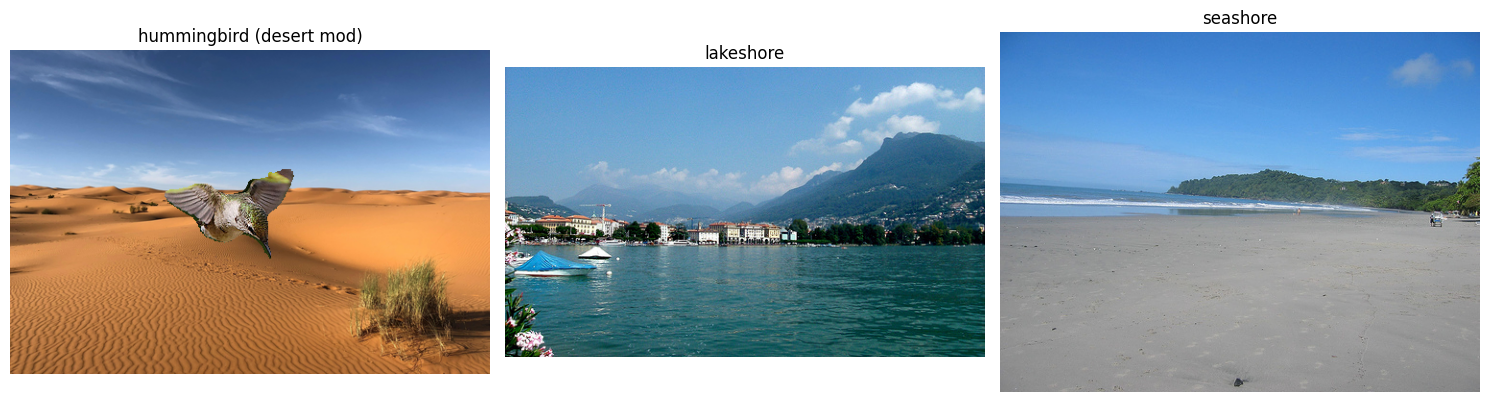
\includegraphics[width=.9\textwidth]{img/94}
	\caption{Od lewej "hummingbird", "lakeshore", "seashore"}
	\label{rys:94}
\end{figure}

\subsection*{Model ConvNeXt}

Model ConvNeXt okazał się zdecydowanie bardziej odporny na modyfikację w kontekście tej klasy. Ciekawym zjawiskiem było częste (15\%) klasyfikowanie ptaka jako wielbłąda dla scenerii pustynnych, co ponownie pokazuję istotny wpływ tła na klasyfikację. Model również traktował inne obiekty 
na zdjęciach jako te porządane, np. dla scenerii miejskiej często klasyfikował zdjęcia tej klasy jako sygnalizacje swietlną, co może wynikać z wysokiego prawdopodobieństwa, że model podczas uczenia widział zdjęcia sygnalizacji świetlnej, na których również występowały ptaki. 

\begin{table}
	\centering
	\begin{tabular}{|c|c|c|c|}
		\hline
		\textbf{Modification Type} & \textbf{Accuracy} & \textbf{Avg Confidence} & \textbf{Most Mistaken} \\
		\hline
		Original & 0.963 & 95.023629 & Jacamar (9) \\
		\hline
		Desert & 0.677 & 73.851502 & Seashore, coast (195) \\
		\hline
		Low Contrast & 0.836 & 83.892216 & Kite (31) \\
		\hline
		City & 0.649 & 63.584482 & Flagpole, flagstaff (34) \\
		\hline
		Sky & 0.789 & 81.238139 & Volcano (48) \\
		\hline
		Jungle & 0.796 & 80.272471 & Greenhouse, nursery (53) \\
		\hline
		No Background & 0.816 & 80.511866 & Vine snake (21) \\
		\hline
		High Contrast & 0.782 & 79.808579 & Kite (47) \\
		\hline
		No Foreground & 0.744 & 69.953177 & Vulture (20) \\
		\hline
		Water & 0.525 & 60.158964 & Albatross, mollymawk (145) \\
		\hline
		Snow & 0.543 & 63.296984 & Snowmobile (151) \\
		\hline
		Indoor & 0.565 & 66.628743 & File, file cabinet (186) \\
		\hline
		Mountain & 0.456 & 54.866228 & Lakeside, lakeshore (121) \\
		\hline
	\end{tabular}
	\caption{Metrics and Confidence Scores for Class 94 (Hummingbird) - ResNet}
	\label{tab:metrics_confidence_class_94_resnet}
\end{table}

\begin{table}
	\centering
	\begin{tabular}{|c|c|c|c|}
		\hline
		\textbf{Modification Type} & \textbf{Accuracy} & \textbf{Avg Confidence} & \textbf{Most Mistaken} \\
		\hline
		Original & 0.995 & 72.907262 & Jacamar (3) \\
		\hline
		Desert & 0.805 & 63.267602 & Arabian camel, dromedary (156) \\
		\hline
		Low Contrast & 0.928 & 57.850450 & Matchstick (14) \\
		\hline
		City & 0.826 & 56.319503 & Traffic light, traffic signal (110) \\
		\hline
		Sky & 0.848 & 57.166515 & Parachute, chute (73) \\
		\hline
		Jungle & 0.859 & 61.211524 & Cliff, drop (73) \\
		\hline
		No Background & 0.933 & 58.181061 & Matchstick (19) \\
		\hline
		High Contrast & 0.911 & 56.167147 & Kite (27) \\
		\hline
		No Foreground & 0.868 & 67.694296 & Jacamar (30) \\
		\hline
		Water & 0.821 & 56.428329 & Albatross, mollymawk (71) \\
		\hline
		Snow & 0.801 & 60.554314 & Lakeside, lakeshore (51) \\
		\hline
		Indoor & 0.718 & 57.200175 & File, file cabinet (123) \\
		\hline
		Mountain & 0.774 & 59.565332 & Valley, vale (73) \\
		\hline
	\end{tabular}
	\caption{Metrics and Confidence Scores for Class 94 (Hummingbird) - ConvNeXt}
	\label{tab:metrics_confidence_class_94_convnext}
\end{table}

\section*{Wnioski dla klasy 285 (Egyptian cat)}

Na podstawie wyników dwóch modeli przedstawionych w \ref*{metrics_confidence_class_285_resnet} i \ref*{metrics_confidence_class_238_convnext}, można wyciągnąć następujące wnioski dotyczące wpływu różnych 
modyfikacji tła na klasyfikację klasy 285 (Egyptian cat) przy użyciu modeli ResNet i ConvNeXt:

\subsection*{Model ResNet}

Dla 5 typów modyfikacji uzyskano lepsze wyniki niż dla oryginalnych zdjęć. W przypadku pozostawienia tła czarnego poprawiono dokładność aż o 7 punktów procentowych, z 78\% do 85\%. Najczęściej myloną klasą, prawie dla każdej modyfikacji była klasas "Tabby cat", która podobnie jak
we wcześniejszym przypadku jest bardzo podobna do klasy przewidywanej. Ciekawym zauważonym zjawiskiem była pomyłka modelu dla scenerii śnieżnej oraz dżungli, gdzie pomylono się na klasę "Tiger cat". Po analizie dostępnych zdjęć treningowych dla klasy tiger cat zauważyłem, że w ich skład 
wchodzą zarówno zdjęcia przedstawiające kota domowego jak i zdjęcia tygrysa. Przykłady zdjęć widnieją na obrazku \ref*{label}

\begin{figure}
	\centering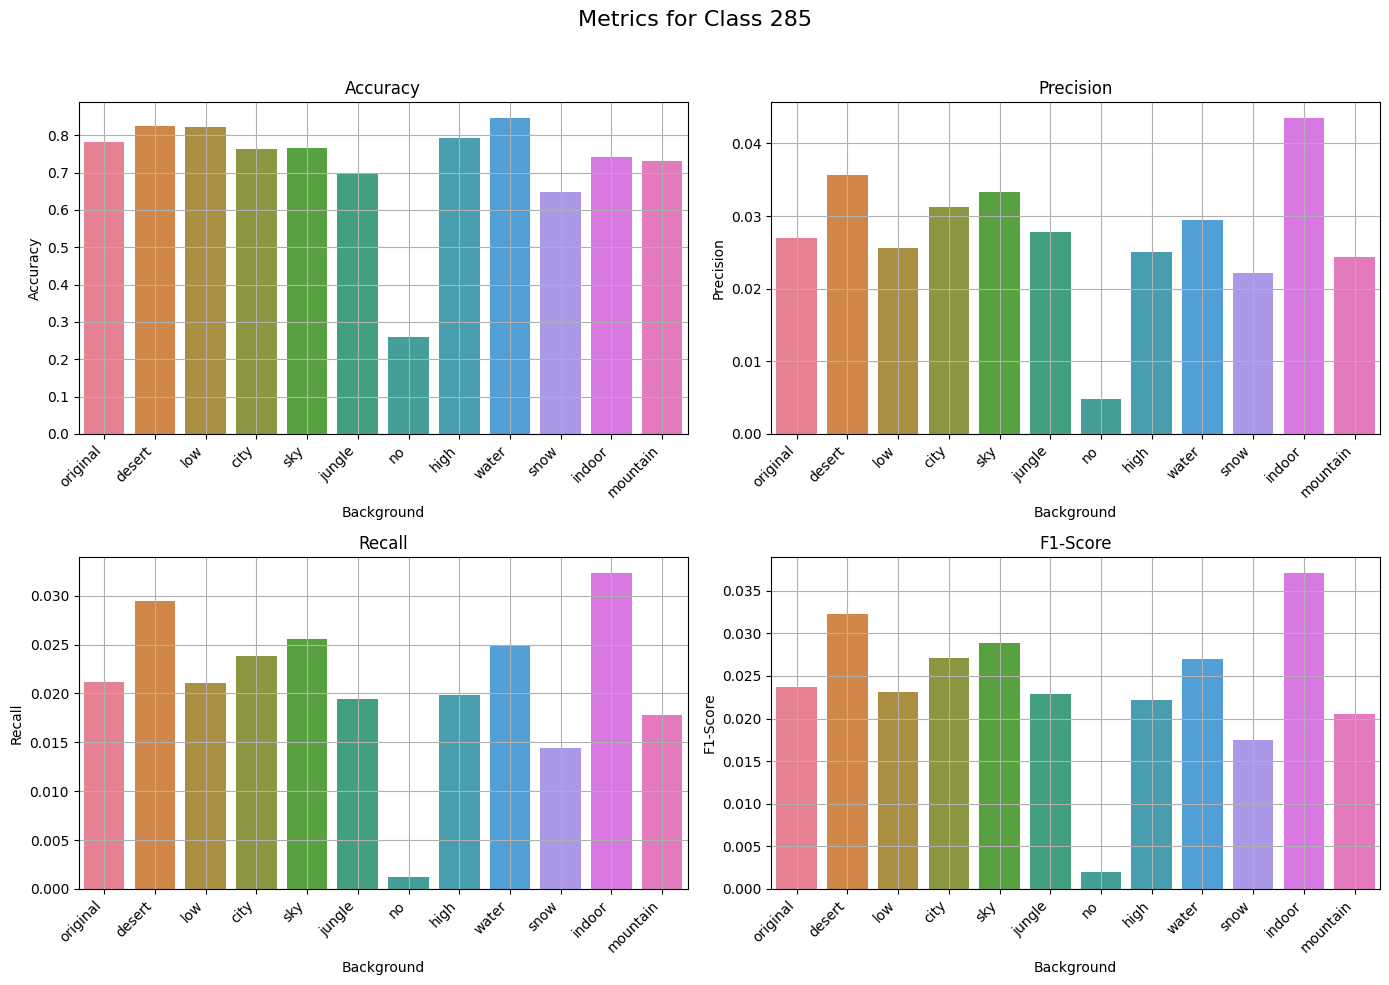
\includegraphics[width=.9\textwidth]{img/285}
	\caption{}
	\label{rys:285}
\end{figure}

\subsection*{Model ConvNeXt}


\begin{table}
	\centering
	\begin{tabular}{|c|c|c|c|}
		\hline
		\textbf{Modification Type} & \textbf{Accuracy} & \textbf{Avg Confidence} & \textbf{Most Mistaken} \\
		\hline
		Original & 0.782 & 73.471966 & Tabby, tabby cat (132) \\
		\hline
		Desert & 0.825 & 76.229713 & Tabby, tabby cat (90) \\
		\hline
		Low Contrast & 0.821 & 78.051673 & Tabby, tabby cat (123) \\
		\hline
		City & 0.763 & 71.972776 & Tabby, tabby cat (136) \\
		\hline
		Sky & 0.766 & 71.577528 & Tabby, tabby cat (119) \\
		\hline
		Jungle & 0.698 & 70.001732 & Tiger cat (136) \\
		\hline
		No Background & 0.847 & 76.844117 & Tabby, tabby cat (85) \\
		\hline
		High Contrast & 0.794 & 77.981898 & Tabby, tabby cat (146) \\
		\hline
		No Foreground & 0.260 & 33.898078 & Quilt, comforter (56) \\
		\hline
		Water & 0.846 & 75.972695 & Tabby, tabby cat (57) \\
		\hline
		Snow & 0.647 & 67.339146 & Tiger cat (121) \\
		\hline
		Indoor & 0.743 & 74.809806 & Tabby, tabby cat (128) \\
		\hline
		Mountain & 0.730 & 67.302426 & Tabby, tabby cat (127) \\
		\hline
	\end{tabular}
	\caption{Metrics and Confidence Scores for Class 285 (Egyptian cat) - ResNet}
	\label{tab:metrics_confidence_class_285_resnet}
\end{table}

\begin{table}
	\centering
	\begin{tabular}{|c|c|c|c|}
		\hline
		\textbf{Modification Type} & \textbf{Accuracy} & \textbf{Avg Confidence} & \textbf{Most Mistaken} \\
		\hline
		Original & 0.875 & 67.470651 & Tabby, tabby cat (83) \\
		\hline
		Desert & 0.840 & 64.843979 & Tabby, tabby cat (96) \\
		\hline
		Low Contrast & 0.842 & 60.234300 & Tabby, tabby cat (112) \\
		\hline
		City & 0.788 & 58.385278 & Tabby, tabby cat (134) \\
		\hline
		Sky & 0.783 & 55.255898 & Tabby, tabby cat (126) \\
		\hline
		Jungle & 0.816 & 59.110254 & Tabby, tabby cat (113) \\
		\hline
		No Background & 0.872 & 63.906281 & Tabby, tabby cat (89) \\
		\hline
		High Contrast & 0.816 & 60.301645 & Tabby, tabby cat (143) \\
		\hline
		No Foreground & 0.301 & 36.188940 & Schipperke (157) \\
		\hline
		Water & 0.862 & 58.187896 & Tabby, tabby cat (87) \\
		\hline
		Snow & 0.823 & 59.457130 & Tabby, tabby cat (114) \\
		\hline
		Indoor & 0.724 & 62.997077 & Bookcase (100) \\
		\hline
		Mountain & 0.829 & 58.399331 & Tabby, tabby cat (87) \\
		\hline
	\end{tabular}
	\caption{Metrics and Confidence Scores for Class 285 (Egyptian cat) - ConvNeXt}
	\label{tab:metrics_confidence_class_285_convnext}
\end{table}

\section*{Wnioski dla klasy 349 (Bighorn sheep)}

Na podstawie wyników przedstawionych w Tabeli X i Tabeli Y, można wyciągnąć następujące wnioski dotyczące wpływu różnych modyfikacji tła na klasyfikację klasy 349 (Bighorn sheep) przy użyciu modeli ResNet i ConvNeXt:

\subsection*{Model ResNet}


\subsection*{Model ConvNeXt}



\begin{table}
	\centering
	\begin{tabular}{|c|c|c|c|}
		\hline
		\textbf{Modification Type} & \textbf{Accuracy} & \textbf{Avg Confidence} & \textbf{Most Mistaken} \\
		\hline
		Original & 0.857 & 76.879462 & Ram, tup (124) \\
		\hline
		Desert & 0.644 & 65.576020 & Seashore, coast (125) \\
		\hline
		Low Contrast & 0.707 & 62.688885 & Ram, tup (103) \\
		\hline
		City & 0.583 & 57.522109 & Ram, tup (171) \\
		\hline
		Sky & 0.501 & 61.268969 & Ram, tup (273) \\
		\hline
		Jungle & 0.471 & 59.756806 & Ram, tup (351) \\
		\hline
		No Background & 0.635 & 57.550804 & Ram, tup (145) \\
		\hline
		High Contrast & 0.583 & 59.381386 & Ram, tup (218) \\
		\hline
		No Foreground & 0.300 & 46.576951 & American black bear, black bear (128) \\
		\hline
		Water & 0.457 & 58.803368 & Ram, tup (329) \\
		\hline
		Snow & 0.783 & 72.009580 & Alp (73) \\
		\hline
		Indoor & 0.467 & 60.394391 & Ram, tup (220) \\
		\hline
		Mountain & 0.725 & 66.198482 & Ram, tup (77) \\
		\hline
	\end{tabular}
	\caption{Metrics and Confidence Scores for Class 349 (Bighorn sheep) - ResNet}
	\label{tab:metrics_confidence_class_349_resnet}
\end{table}

\begin{table}
	\centering
	\begin{tabular}{|c|c|c|c|}
		\hline
		\textbf{Modification Type} & \textbf{Accuracy} & \textbf{Avg Confidence} & \textbf{Most Mistaken} \\
		\hline
		Original & 0.908 & 56.144302 & Ram, tup (89) \\
		\hline
		Desert & 0.739 & 53.343471 & Arabian camel, dromedary (219) \\
		\hline
		Low Contrast & 0.792 & 43.160569 & Ram, tup (110) \\
		\hline
		City & 0.814 & 48.102590 & Traffic light, traffic signal (103) \\
		\hline
		Sky & 0.660 & 44.070363 & Ram, tup (151) \\
		\hline
		Jungle & 0.709 & 47.144147 & Ram, tup (133) \\
		\hline
		No Background & 0.776 & 42.662816 & Ram, tup (88) \\
		\hline
		High Contrast & 0.786 & 42.740627 & Ram, tup (89) \\
		\hline
		No Foreground & 0.369 & 41.866028 & American black bear, black bear (171) \\
		\hline
		Water & 0.714 & 44.812545 & Ram, tup (147) \\
		\hline
		Snow & 0.878 & 55.639899 & Lakeside, lakeshore (79) \\
		\hline
		Indoor & 0.715 & 51.461317 & File, file cabinet (155) \\
		\hline
		Mountain & 0.826 & 53.093244 & Valley, vale (89) \\
		\hline
	\end{tabular}
	\caption{Metrics and Confidence Scores for Class 349 (Bighorn sheep) - ConvNeXt}
	\label{tab:metrics_confidence_class_349_convnext}
\end{table}

\section*{Wnioski dla klasy 229 (Old English sheepdog)}

Na podstawie wyników przedstawionych w Tabeli X i Tabeli Y, można wyciągnąć następujące wnioski dotyczące wpływu różnych modyfikacji tła na klasyfikację klasy 229 (Old English sheepdog) przy użyciu modeli ResNet i ConvNeXt:

\subsection*{Model ResNet}


\subsection*{Model ConvNeXt}



\begin{table}
	\centering
	\begin{tabular}{|c|c|c|c|}
		\hline
		\textbf{Modification Type} & \textbf{Accuracy} & \textbf{Avg Confidence} & \textbf{Most Mistaken} \\
		\hline
		Original & 0.941 & 88.632230 & Tibetan terrier, chrysanthemum dog (9) \\
		\hline
		Desert & 0.801 & 80.359347 & Seashore, coast (64) \\
		\hline
		Low Contrast & 0.785 & 77.904651 & Sealyham terrier, Sealyham (39) \\
		\hline
		City & 0.765 & 74.680369 & Cab, hack (21) \\
		\hline
		Sky & 0.718 & 74.347288 & Volcano (63) \\
		\hline
		Jungle & 0.782 & 75.977385 & Greenhouse, nursery (32) \\
		\hline
		No Background & 0.709 & 71.070938 & Sealyham terrier, Sealyham (56) \\
		\hline
		High Contrast & 0.760 & 75.577558 & Sealyham terrier, Sealyham (47) \\
		\hline
		No Foreground & 0.071 & 31.629389 & American black bear, black bear (69) \\
		\hline
		Water & 0.758 & 76.056336 & Albatross, mollymawk (78) \\
		\hline
		Snow & 0.803 & 80.582623 & Alp (44) \\
		\hline
		Indoor & 0.824 & 84.001364 & File, file cabinet (60) \\
		\hline
		Mountain & 0.715 & 70.130826 & Valley, vale (44) \\
		\hline
	\end{tabular}
	\caption{Metrics and Confidence Scores for Class 229 (Old English sheepdog) - ResNet}
	\label{tab:metrics_confidence_class_229_resnet}
\end{table}

\begin{table}
	\centering
	\begin{tabular}{|c|c|c|c|}
		\hline
		\textbf{Modification Type} & \textbf{Accuracy} & \textbf{Avg Confidence} & \textbf{Most Mistaken} \\
		\hline
		Original & 0.987 & 74.735155 & Collie (2) \\
		\hline
		Desert & 0.871 & 66.845438 & Arabian camel, dromedary (96) \\
		\hline
		Low Contrast & 0.910 & 60.380093 & Matchstick (25) \\
		\hline
		City & 0.882 & 63.133430 & Traffic light, traffic signal (52) \\
		\hline
		Sky & 0.824 & 56.268607 & Volcano (77) \\
		\hline
		Jungle & 0.890 & 64.798835 & Cliff, drop (43) \\
		\hline
		No Background & 0.869 & 59.633430 & Matchstick (26) \\
		\hline
		High Contrast & 0.891 & 59.879026 & Matchstick (28) \\
		\hline
		No Foreground & 0.109 & 32.475152 & Newfoundland, Newfoundland dog (188) \\
		\hline
		Water & 0.879 & 60.280609 & Grey whale, gray whale (32) \\
		\hline
		Snow & 0.896 & 64.967973 & Lakeside, lakeshore (38) \\
		\hline
		Indoor & 0.867 & 69.414455 & Bookcase (58) \\
		\hline
		Mountain & 0.856 & 62.675450 & Valley, vale (44) \\
		\hline
	\end{tabular}
	\caption{Metrics and Confidence Scores for Class 229 (Old English sheepdog) - ConvNeXt}
	\label{tab:metrics_confidence_class_229_convnext}
\end{table}

\section*{Wnioski dla klasy 283 (Persian cat)}

Na podstawie wyników przedstawionych w Tabeli X i Tabeli Y, można wyciągnąć następujące wnioski dotyczące wpływu różnych modyfikacji tła na klasyfikację klasy 283 (Persian cat) przy użyciu modeli ResNet i ConvNeXt:

\subsection*{Model ResNet}


\subsection*{Model ConvNeXt}


\begin{table}
	\centering
	\begin{tabular}{|c|c|c|c|}
		\hline
		\textbf{Modification Type} & \textbf{Accuracy} & \textbf{Avg Confidence} & \textbf{Most Mistaken} \\
		\hline
		Original & 0.964 & 93.028729 & Angora, Angora rabbit (9) \\
		\hline
		Desert & 0.848 & 83.349976 & Seashore, coast (41) \\
		\hline
		Low Contrast & 0.855 & 83.713232 & Tabby, tabby cat (26) \\
		\hline
		City & 0.877 & 84.163735 & Tabby, tabby cat (15) \\
		\hline
		Sky & 0.821 & 82.203083 & Volcano (52) \\
		\hline
		Jungle & 0.831 & 81.888781 & Greenhouse, nursery (25) \\
		\hline
		No Background & 0.844 & 81.940165 & Egyptian cat (19) \\
		\hline
		High Contrast & 0.853 & 84.050749 & Tabby, tabby cat (30) \\
		\hline
		No Foreground & 0.025 & 23.772934 & Quilt, comforter (70) \\
		\hline
		Water & 0.821 & 79.093091 & Albatross, mollymawk (23) \\
		\hline
		Snow & 0.829 & 82.849727 & Alp (31) \\
		\hline
		Indoor & 0.879 & 87.654082 & File, file cabinet (41) \\
		\hline
		Mountain & 0.794 & 77.893145 & Valley, vale (25) \\
		\hline
	\end{tabular}
	\caption{Metrics and Confidence Scores for Class 283 (Persian cat) - ResNet}
	\label{tab:metrics_confidence_class_283_resnet}
\end{table}

\begin{table}
	\centering
	\begin{tabular}{|c|c|c|c|}
		\hline
		\textbf{Modification Type} & \textbf{Accuracy} & \textbf{Avg Confidence} & \textbf{Most Mistaken} \\
		\hline
		Original & 0.991 & 75.141474 & Feather boa, boa (1) \\
		\hline
		Desert & 0.914 & 70.630613 & Arabian camel, dromedary (65) \\
		\hline
		Low Contrast & 0.947 & 66.190509 & Matchstick (13) \\
		\hline
		City & 0.936 & 68.423853 & Traffic light, traffic signal (36) \\
		\hline
		Sky & 0.887 & 63.020165 & Volcano (54) \\
		\hline
		Jungle & 0.925 & 67.672465 & Cliff, drop (24) \\
		\hline
		No Background & 0.937 & 68.087824 & Matchstick (13) \\
		\hline
		High Contrast & 0.942 & 68.444946 & Corkscrew, bottle screw (13) \\
		\hline
		No Foreground & 0.061 & 25.145970 & Schipperke (96) \\
		\hline
		Water & 0.906 & 59.895699 & Grey whale, gray whale (19) \\
		\hline
		Snow & 0.925 & 67.393982 & Lakeside, lakeshore (23) \\
		\hline
		Indoor & 0.907 & 72.101543 & Bookcase (37) \\
		\hline
		Mountain & 0.916 & 67.004423 & Valley, vale (26) \\
		\hline
	\end{tabular}
	\caption{Metrics and Confidence Scores for Class 283 (Persian cat) - ConvNeXt}
	\label{tab:metrics_confidence_class_283_convnext}
\end{table}

\section*{Wnioski dla klasy 13 (junco, snowbird)}

Na podstawie wyników przedstawionych w Tabeli X i Tabeli Y, można wyciągnąć następujące wnioski dotyczące wpływu różnych modyfikacji tła na klasyfikację klasy 13 (junco, snowbird) przy użyciu modeli ResNet i ConvNeXt:

\subsection*{Model ResNet}


\subsection*{Model ConvNeXt}


\begin{table}
	\centering
	\begin{tabular}{|c|c|c|c|}
		\hline
		\textbf{Modification Type} & \textbf{Accuracy} & \textbf{Avg Confidence} & \textbf{Most Mistaken} \\
		\hline
		Original & 0.976 & 95.314826 & House finch, linnet (7) \\
		\hline
		Desert & 0.839 & 81.161059 & Seashore, coast (97) \\
		\hline
		Low Contrast & 0.877 & 86.390556 & Brambling, Fringilla montifringilla (26) \\
		\hline
		City & 0.842 & 75.437180 & House finch, linnet (30) \\
		\hline
		Sky & 0.842 & 83.426079 & Volcano (46) \\
		\hline
		Jungle & 0.920 & 90.342285 & Bittern (11) \\
		\hline
		No Background & 0.858 & 84.076516 & Electric ray, crampfish (33) \\
		\hline
		High Contrast & 0.896 & 87.080903 & Kite (15) \\
		\hline
		No Foreground & 0.362 & 51.447448 & Water ouzel, dipper (216) \\
		\hline
		Water & 0.716 & 61.873004 & Albatross, mollymawk (124) \\
		\hline
		Snow & 0.831 & 83.117293 & Snowmobile (66) \\
		\hline
		Indoor & 0.676 & 68.064425 & File, file cabinet (132) \\
		\hline
		Mountain & 0.797 & 76.813323 & Lakeside, lakeshore (60) \\
		\hline
	\end{tabular}
	\caption{Metrics and Confidence Scores for Class 13 (junco, snowbird) - ResNet}
	\label{tab:metrics_confidence_class_13_resnet}
\end{table}

\begin{table}
	\centering
	\begin{tabular}{|c|c|c|c|}
		\hline
		\textbf{Modification Type} & \textbf{Accuracy} & \textbf{Avg Confidence} & \textbf{Most Mistaken} \\
		\hline
		Original & 1.000 & 68.830393 & None \\
		\hline
		Desert & 0.915 & 64.330613 & Arabian camel, dromedary (75) \\
		\hline
		Low Contrast & 0.982 & 58.656551 & Chickadee (3) \\
		\hline
		City & 0.888 & 58.006623 & Traffic light, traffic signal (67) \\
		\hline
		Sky & 0.935 & 60.091004 & Parachute, chute (31) \\
		\hline
		Jungle & 0.954 & 60.319277 & Cliff, drop (16) \\
		\hline
		No Background & 0.971 & 58.450551 & Water ouzel, dipper (5) \\
		\hline
		High Contrast & 0.983 & 58.033862 & Brambling, Fringilla montifringilla (2) \\
		\hline
		No Foreground & 0.460 & 37.770219 & Magpie (187) \\
		\hline
		Water & 0.935 & 58.536078 & Albatross, mollymawk (27) \\
		\hline
		Snow & 0.929 & 61.614732 & Lakeside, lakeshore (15) \\
		\hline
		Indoor & 0.837 & 59.676453 & File, file cabinet (67) \\
		\hline
		Mountain & 0.930 & 64.416702 & Valley, vale (16) \\
		\hline
	\end{tabular}
	\caption{Metrics and Confidence Scores for Class 13 (junco, snowbird) - ConvNeXt}
	\label{tab:metrics_confidence_class_13_convnext}
\end{table}

\section*{Wnioski dla klasy 235 (German shepherd)}

Na podstawie wyników przedstawionych w Tabeli X i Tabeli Y, można wyciągnąć następujące wnioski dotyczące wpływu różnych modyfikacji tła na klasyfikację klasy 235 (German shepherd) przy użyciu modeli ResNet i ConvNeXt:

\subsection*{Model ResNet}


\subsection*{Model ConvNeXt}


\begin{table}
	\centering
	\begin{tabular}{|c|c|c|c|}
		\hline
		\textbf{Modification Type} & \textbf{Accuracy} & \textbf{Avg Confidence} & \textbf{Most Mistaken} \\
		\hline
		Original & 0.874 & 82.761220 & Malinois (40) \\
		\hline
		Desert & 0.705 & 72.608107 & Norwegian elkhound, elkhound (103) \\
		\hline
		Low Contrast & 0.806 & 77.606469 & Malinois (41) \\
		\hline
		City & 0.821 & 77.924239 & Malinois (41) \\
		\hline
		Sky & 0.787 & 75.390463 & Norwegian elkhound, elkhound (38) \\
		\hline
		Jungle & 0.788 & 76.892591 & Malinois (53) \\
		\hline
		No Background & 0.705 & 67.817178 & Coyot
		Model ResNet osiągnął wysoką dokładność 0.981 na oryginalnych obrazach, co wskazuje na jego skuteczność w klasyfikacji klasy 15 w standardowych warunkach. Średnia pewność wynosiła 96.633280, co jest bardzo wysoką wartością, potwierdzającą pewność modelu przy klasyfikacji.
		
		Znaczący spadek dokładności został zanotowany przy modyfikacjach tła. Najniższa dokładność została zanotowana przy modyfikacji "No Foreground" (0.023), co wskazuje na dużą trudność modelu w klasyfikacji obiektów bez tła. Inne modyfikacje, takie jak "Desert" (0.830), "Low Contrast" (0.883), i "City" (0.909), również obniżyły dokładność modelu, co sugeruje, że zmiany w tle mogą negatywnie wpływać na wydajność modelu.
		
		Model najczęściej mylił klasę 15 z "Hummingbird" przy większości modyfikacji tła. Wyjątek stanowiła modyfikacja "No Foreground", gdzie model najczęściej mylił klasę z "Magpie".e, prairie wolf (32) \\
		\hline
		High Contrast & 0.819 & 80.306382 & Malinois (39) \\
		\hline
		No Foreground & 0.005 & 36.099894 & Egyptian cat (140) \\
		\hline
		Water & 0.814 & 76.923269 & Malinois (45) \\
		\hline
		Snow & 0.780 & 78.109030 & Malinois (52) \\
		\hline
		Indoor & 0.725 & 74.028374 & Norwegian elkhound, elkhound (54) \\
		\hline
		Mountain & 0.666 & 65.790195 & Malinois (65) \\
		\hline
	\end{tabular}
	\caption{Metrics and Confidence Scores for Class 235 (German shepherd) - ResNet}
	\label{tab:metrics_confidence_class_235_resnet}
\end{table}

\begin{table}
	\centering
	\begin{tabular}{|c|c|c|c|}
		\hline
		\textbf{Modification Type} & \textbf{Accuracy} & \textbf{Avg Confidence} & \textbf{Most Mistaken} \\
		\hline
		Original & 0.961 & 69.949959 & Malinois (10) \\
		\hline
		Desert & 0.844 & 62.162412 & Arabian camel, dromedary (83) \\
		\hline
		Low Contrast & 0.919 & 61.204567 & Malinois (17) \\
		\hline
		City & 0.867 & 59.458822 & Traffic light, traffic signal (23) \\
		\hline
		Sky & 0.873 & 62.404542 & Norwegian elkhound, elkhound (30) \\
		\hline
		Jungle & 0.908 & 64.776667 & Cliff, drop (14) \\
		\hline
		No Background & 0.886 & 60.678388 & Malinois (10) \\
		\hline
		High Contrast & 0.919 & 61.661308 & Malinois (17) \\
		\hline
		No Foreground & 0.042 & 38.284114 & Schipperke (239) \\
		\hline
		Water & 0.922 & 62.505798 & Norwegian elkhound, elkhound (14) \\
		\hline
		Snow & 0.890 & 63.506425 & Norwegian elkhound, elkhound (29) \\
		\hline
		Indoor & 0.800 & 64.582883 & Bookcase (65) \\
		\hline
		Mountain & 0.847 & 61.401422 & Norwegian elkhound, elkhound (36) \\
		\hline
	\end{tabular}
	\caption{Metrics and Confidence Scores for Class 235 (German shepherd) - ConvNeXt}
	\label{tab:metrics_confidence_class_235_convnext}
\end{table}

\section*{Wnioski dla klasy 15 (American robin)}

Na podstawie wyników przedstawionych w Tabeli X i Tabeli Y, można wyciągnąć następujące wnioski dotyczące wpływu różnych modyfikacji tła na klasyfikację klasy 15 (American robin) przy użyciu modeli ResNet i ConvNeXt:

\subsection*{Model ResNet}


\subsection*{Model ConvNeXt}


\begin{table}
	\centering
	\begin{tabular}{|c|c|c|c|}
		\hline
		\textbf{Modification Type} & \textbf{Accuracy} & \textbf{Avg Confidence} & \textbf{Most Mistaken} \\
		\hline
		Original & 0.981 & 96.633280 & Hummingbird (2) \\
		\hline
		Desert & 0.830 & 81.119547 & Seashore, coast (87) \\
		\hline
		Low Contrast & 0.883 & 89.243569 & Brambling, Fringilla montifringilla (27) \\
		\hline
		City & 0.909 & 87.792362 & Obelisk (11) \\
		\hline
		Sky & 0.908 & 89.332178 & Volcano (15) \\
		\hline
		Jungle & 0.945 & 92.875282 & Greenhouse, nursery (12) \\
		\hline
		No Background & 0.872 & 86.418034 & Brambling, Fringilla montifringilla (18) \\
		\hline
		High Contrast & 0.903 & 89.287356 & Kite (16) \\
		\hline
		No Foreground & 0.023 & 49.667002 & Magpie (226) \\
		\hline
		Water & 0.802 & 73.219416 & Snorkel (23) \\
		\hline
		Snow & 0.897 & 88.912560 & Snowmobile (49) \\
		\hline
		Indoor & 0.678 & 69.680563 & File, file cabinet (85) \\
		\hline
		Mountain & 0.879 & 88.491847 & Lakeside, lakeshore (33) \\
		\hline
	\end{tabular}
	\caption{Metrics and Confidence Scores for Class 15 (American robin) - ResNet}
	\label{tab:metrics_confidence_class_15_resnet}
\end{table}

\begin{table}
	\centering
	\begin{tabular}{|c|c|c|c|}
		\hline
		\textbf{Modification Type} & \textbf{Accuracy} & \textbf{Avg Confidence} & \textbf{Most Mistaken} \\
		\hline
		Original & 0.997 & 68.229925 & Worm fence, snake fence (1) \\
		\hline
		Desert & 0.905 & 58.872557 & Arabian camel, dromedary (73) \\
		\hline
		Low Contrast & 0.968 & 59.050634 & House finch, linnet (4) \\
		\hline
		City & 0.942 & 59.546505 & Traffic light, traffic signal (34) \\
		\hline
		Sky & 0.948 & 60.918330 & Parachute, chute (20) \\
		\hline
		Jungle & 0.960 & 59.782053 & Cliff, drop (17) \\
		\hline
		No Background & 0.951 & 56.262251 & Hummingbird (11) \\
		\hline
		High Contrast & 0.963 & 58.630182 & Water ouzel, dipper (7) \\
		\hline
		No Foreground & 0.052 & 39.404290 & Magpie (482) \\
		\hline
		Water & 0.941 & 57.640282 & Grey whale, gray whale (15) \\
		\hline
		Snow & 0.952 & 63.954396 & Snowmobile (17) \\
		\hline
		Indoor & 0.858 & 58.543296 & Bookcase (62) \\
		\hline
		Mountain & 0.941 & 63.929843 & Valley, vale (14) \\
		\hline
	\end{tabular}
	\caption{Metrics and Confidence Scores for Class 15 (American robin) - ConvNeXt}
	\label{tab:metrics_confidence_class_15_convnext}
\end{table}
